
\documentclass{article}
\usepackage{iclr2027_conference,times}

\IfFileExists{math_commands.tex}{\input{math_commands.tex}}{}

\usepackage{hyperref}
\usepackage{url}
\usepackage{amsmath,amssymb,booktabs,graphicx,microtype,xcolor,multirow}

\newcommand{\TODO}[1]{\textcolor{red}{[TODO: #1]}}

\title{S-LoRA: Squared LoRA via Exact Row-Space\\Factorization for
       Parameter-Efficient Fine-Tuning}

\author{Hiep Nguyen \\
Independent Researcher \\
\texttt{hiepdema26@gmail.com}
}

\begin{document}

\maketitle

\begin{abstract}
Low-rank adaptation (LoRA) has become a standard approach for parameter-efficient fine-tuning (PEFT), but its parameter cost remains proportional to the full dimensions of the adapted weight matrix. This becomes particularly inefficient for the highly non-square projection matrices found in modern architectures, where one dimension may be substantially larger than the other despite the weight itself having limited intrinsic capacity. We introduce \textbf{S-LoRA} (Squared LoRA), a simple reparameterization of LoRA that exploits this asymmetry without discarding any pretrained information. Instead of applying a low-rank update to the original weight, S-LoRA exactly factorizes each non-square weight into a frozen rectangular factor and a square factor initialized from its pretrained values, and performs adaptation exclusively on the square factor. This construction is lossless at initialization, preserves the full pretrained function, and confines the adaptation to the pretrained row space of the original weight. Because the trainable factor is square, S-LoRA reduces the parameter cost of dimension-scaled adapters in proportion to the aspect ratio of the original weight, while the resulting adapted weight can be merged into a single matrix with no additional inference cost. On E2E NLG, fine-tuning only the key and value projections of Qwen2.5-1.5B, S-LoRA reaches $65.2$ BLEU with only $0.057$M trainable parameters, surpassing unconstrained training of the same projections ($64.3$ BLEU with $22.0$M parameters) and matching LoRA's performance with substantially fewer parameters. At matched parameter budgets, S-LoRA improves over LoRA by up to $2.75$ BLEU, with statistically significant gains of $4.0\sigma$, $2.7\sigma$, and $1.3\sigma$ at representative budgets. These results show that exploiting the pretrained geometry of non-square weights provides a simple and effective way to improve the parameter efficiency of LoRA, particularly in the low-budget regime. More broadly, S-LoRA offers a drop-in reparameterization of LoRA that preserves pretrained structure while substantially reducing the cost of adaptation.
\end{abstract}

\section{Introduction}

Adapting a pretrained language model to a downstream task by updating all of
its weights is rarely practical, and the field has converged on a common
answer: keep $W_0$ frozen and learn a small additive correction. LoRA
\citep{hu2022lora} parameterizes that correction as a rank-$r$ product $BA$;
the many variants that followed change how $B$ and $A$ are initialized
\citep{meng2024pissa,wang2024milora}, decomposed \citep{liu2024dora},
allocated \citep{zhang2023adalora}, or shared
\citep{kopiczko2024vera,balazy2024loraxs}, but they all inherit the same
additive skeleton $W_0 + \Delta W$. The cost of every such adapter is
$O(r(n+m))$: it scales with \emph{both} dimensions of the weight it adapts.%
\footnote{The name S-LoRA has previously been used by \citet{sheng2024slora}
for a serving system that multiplexes thousands of concurrent LoRA adapters.
That work addresses inference-time memory management and is unrelated to the
reparameterization studied here; we adopt the name for its mnemonic value
(\emph{squared}) and note the collision explicitly.}

That scaling is wasteful for lopsided matrices, and modern architectures are
full of them. Grouped-query attention \citep{ainslie2023gqa} deliberately
compresses the key and value projections: in Qwen2.5-1.5B
\citep{qwen2024qwen25} they map $1536$ inputs to $256$ outputs, an aspect ratio
of six. An adapter that pays for the long dimension is paying for capacity the
layer itself does not have. The obvious remedy --- adapt a smaller object ---
runs into a second problem: the small object must still carry pretrained
information, or methods that exploit pretrained structure
\citep{liu2024dora,meng2024pissa} have nothing to attach to. Work that builds
adapters from the rows and columns of $W_0$ itself
\citep{wang2025pmss,fawi2024curlora} comes close, but the trainable object is
still a zero-initialized delta.

We take a different route: replace the layer with an exact factorization
instead of adding to it. Column-pivoted QR \citep{businger1965pivotedqr}
selects $k=\min(n,m)$ columns of $W_0$ that are as well-conditioned as the
greedy criterion can find, and the remaining columns are written exactly in
terms of them --- the interpolative decomposition \citep{cheng2005id}. The
identity block costs nothing to store or apply; it is an index selection, not
a matmul. The reparameterized layer therefore has the same parameter count and
the same FLOP count as the original, and folds back into a single matrix at
deployment. What changes is what is adaptable: the trainable object is now a
square $k\times k$ matrix that still holds pretrained values, so the entire
adapter toolbox applies to it, each tool becoming cheaper by $(1+a)/2$ where
$a=\max(n,m)/k$.

Constraining $\Delta W$ this way is not free, and its price depends on the
budget it is spent under, on the model, and on the task. On Qwen2.5-1.5B
fine-tuned for E2E NLG \citep{novikova2017e2e} with only the key and value
projections adapted, the constraint behaves as a regularizer in the low-budget
regime: quality saturates at rank two --- $0.057$M trainable parameters, under
$0.004\%$ of the model --- and already exceeds what unconstrained training of
those same two matrices achieves with $384\times$ more parameters. At matched
budget the lead over LoRA is $2.75$ BLEU near $0.1$M, narrowing to $0.72$ by
$0.4$M and inverting at rank one.

That advantage does not survive scale. On Mistral-7B \citep{jiang2023mistral}
fine-tuned on MetaMathQA \citep{yu2024metamath} at a matched budget of $167$M
parameters --- the budget at which LoRA and PiSSA are evaluated in the
literature --- S-LoRA reaches $61.94\%$ on GSM8K against LoRA's $72.02\%$, and
$13.30\%$ on MATH against $22.12\%$, losing on all seven MATH subjects. We
report this negative result in full (Section~\ref{sec:scale}) because the same
pipeline reproduces and exceeds the published LoRA baselines, which rules out
implementation error as the explanation. The honest summary is that the
row-space constraint is a favorable trade in a narrow regime and a costly one
outside it, and the boundary is not yet characterized.

\paragraph{Contributions.}
\begin{itemize}
  \item An exact, parameter-preserving reparameterization of non-square weights
        via interpolative decomposition, with a closed-form cost advantage
        $(1+a)/2$ for dimension-dependent adapters and $a$ for full
        fine-tuning.
  \item An analysis showing that adapting the square factor is equivalent to
        preconditioned gradient descent on the original weight,
        $\Delta W=-\eta\,(\partial L/\partial W)(P^{\top}P)$, with the
        preconditioner reducing to an orthogonal projector exactly when the
        basis is orthonormal.
  \item A controlled comparison against LoRA, an unconstrained upper bound, and
        the zero-shot floor across five parameter budgets spanning $16\times$,
        with two to three seeds per configuration.
  \item A negative scaling result at 7B with a validated pipeline, delimiting
        where the constraint helps and where it does not.
\end{itemize}

\section{Related Work}

\paragraph{Additive low-rank adapters.}
LoRA \citep{hu2022lora} descends from adapter layers
\citep{houlsby2019adapter} and prefix tuning \citep{li2021prefix}, and rests on
the observation that fine-tuning updates have low intrinsic dimension
\citep{aghajanyan2021intrinsic}. Subsequent work keeps the additive form and
varies its ingredients: PiSSA \citep{meng2024pissa} initializes $B,A$ from the
principal singular directions of $W_0$ and MiLoRA \citep{wang2024milora} from
the minor ones; DoRA \citep{liu2024dora} separates magnitude from direction;
AdaLoRA \citep{zhang2023adalora} reallocates rank across layers; VeRA
\citep{kopiczko2024vera} freezes random $B,A$ and trains only scaling vectors;
LoRA-XS \citep{balazy2024loraxs} freezes SVD bases and trains an $r\times r$
core; LoRA-FA \citep{zhang2023lorafa} freezes $A$ alone. S-LoRA differs in
kind rather than degree: it is multiplicative, not additive, and the object it
adapts retains pretrained values rather than starting at zero.

\paragraph{Skeleton and CUR-based adapters.}
The closest neighbours build the adapter from the rows and columns of $W_0$
itself, following CUR decomposition \citep{mahoney2009cur}. PMSS
\citep{wang2025pmss} uses the same column-pivoted QR criterion we do, and also
states a subspace constraint; CURLoRA \citep{fawi2024curlora} uses inverted
leverage scores. Three differences matter. PMSS freezes \emph{both} the column
factor $C=W_0(:,J)$ and the row factor $R=W_0(K,:)$ and trains a small $U$
between them, giving a two-sided constraint $\Delta W=CUR$; S-LoRA freezes one
side only. PMSS discards the interpolation matrix entirely --- its Algorithm 1
returns index vectors and never forms it --- so pivoted QR serves purely as a
selection heuristic, whereas we use the factorization it produces. Finally,
PMSS's parameter count $c\cdot r$ is independent of $n$ and $m$, so the
$(1+a)/2$ saving does not apply to it and must not be quoted against it.

\paragraph{Structured alternatives to low rank.}
A parallel line replaces the low-rank prior with a different structural one:
Kronecker factorizations \citep{edalati2022krona}, butterfly and block-diagonal
products \citep{dao2022monarch}, and orthogonal constraints
\citep{qiu2023oft}. These are complementary to our contribution --- they
restructure $\Delta W$, while we restructure the layer that $\Delta W$ attaches
to --- and composing them with the square factor is straightforward, since any
adapter that applies to an $n\times m$ weight applies to a $k\times k$ one.

\section{Method}

\subsection{Notation}
A linear layer maps $x\in\mathbb{R}^{m}$ to $y=W_0x$ with
$W_0\in\mathbb{R}^{n\times m}$ frozen and $n\neq m$. Write
\[
  k=\min(n,m),\qquad a=\frac{\max(n,m)}{k}\ \ge 1,
\]
so $W_0$ holds $nm=ak^2$ entries, and LoRA's correction
$\Delta W=\tfrac{\alpha}{r}BA$, with $B\in\mathbb{R}^{n\times r}$ and
$A\in\mathbb{R}^{r\times m}$, costs $r(n+m)=rk(1+a)$ parameters per layer.
Every quantity below is per layer; $\langle\cdot,\cdot\rangle$ is the Frobenius
inner product; $[\,A\mid B\,]$ and $[\,A\,;B\,]$ denote horizontal and vertical
concatenation.

\begin{figure}[t]
\centering
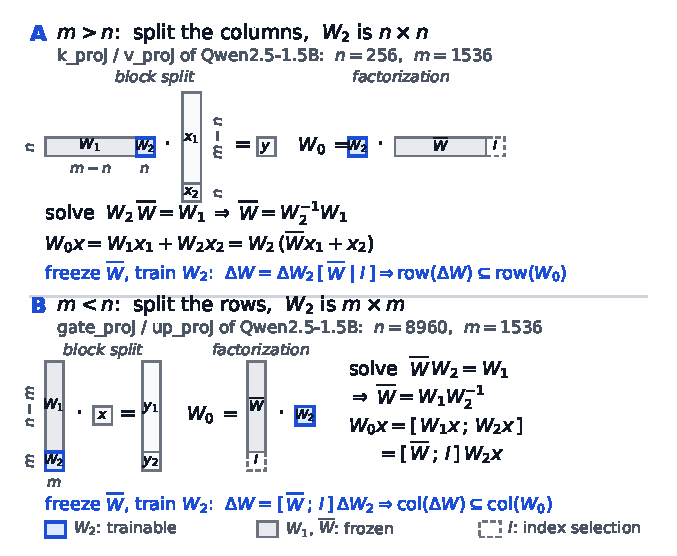
\includegraphics[width=\textwidth]{fig_orientations.pdf}
\caption{Splitting a non-square weight. \textbf{(A)} When $m>n$ the columns
split, $W_0=[\,W_1\mid W_2\,]$ with $W_2$ square, and solving
$W_2\overline{W}=W_1$ gives $W_0=W_2[\,\overline{W}\mid I\,]$: the input is
mixed \emph{before} the square factor, so the update stays in
$\operatorname{row}(W_0)$. \textbf{(B)} When $m<n$ the rows split,
$W_0=[\,W_1\,;W_2\,]$, and solving $\overline{W}W_2=W_1$ gives
$W_0=[\,\overline{W}\,;I\,]W_2$: the output is expanded \emph{after} it, so the
update stays in $\operatorname{col}(W_0)$. Blue marks $W_2$, the only object
adaptation touches and one that still holds pretrained values; grey marks the
frozen blocks; the dashed identity is an index selection costing neither
parameters nor FLOPs. Rectangles are drawn to the true aspect ratios of the
layers named.}
\label{fig:orient}
\end{figure}

\subsection{Splitting a non-square weight}
\label{sec:split}

\paragraph{More inputs than outputs ($m>n$, $k=n$).}
Split the columns of the weight, and the entries of $x$ conformally
(Figure~\ref{fig:orient}A):
\[
  W_0=[\,W_1 \mid W_2\,],\qquad
  W_1\in\mathbb{R}^{n\times(m-n)},\quad W_2\in\mathbb{R}^{n\times n},
  \qquad x=[\,x_1\,;x_2\,].
\]
Whenever the square block $W_2$ is nonsingular, the rectangular block is
determined by it: solving
\begin{equation}
  W_2\,\overline{W}=W_1
  \qquad\Longleftrightarrow\qquad
  \overline{W}=W_2^{-1}W_1\in\mathbb{R}^{n\times(m-n)}
  \label{eq:solve-wide}
\end{equation}
rewrites the layer with no approximation whatsoever,
\begin{equation}
  W_0x \;=\; W_1x_1+W_2x_2 \;=\; W_2\bigl(\overline{W}x_1+x_2\bigr),
  \qquad\text{that is}\qquad
  W_0 \;=\; W_2\,[\,\overline{W}\mid I_n\,].
  \label{eq:wide}
\end{equation}

\paragraph{More outputs than inputs ($n>m$, $k=m$).}
Split the rows instead, and $y$ conformally (Figure~\ref{fig:orient}B). Now the
square block multiplies from the right, so the solve transposes:
\begin{equation}
  \overline{W}\,W_2=W_1
  \quad\Longleftrightarrow\quad
  \overline{W}=W_1W_2^{-1},
  \qquad\text{giving}\qquad
  W_0 \;=\; [\,\overline{W}\,;I_m\,]\,W_2 .
  \label{eq:tall}
\end{equation}
In both cases the layer has been rewritten as a square factor $W_2$ carrying
pretrained values, multiplied by a rectangular factor that contains an identity
block; adaptation is applied to $W_2$ and $\overline{W}$ is frozen. Writing
\begin{equation}
  P=[\,\overline{W}\mid I_n\,]\ \ (m>n),
  \qquad
  P=[\,\overline{W}\,;I_m\,]\ \ (n>m),
  \qquad
  W_0=W_2P \ \text{ or } \ W_0=PW_2,
  \label{eq:P}
\end{equation}
lets the two cases be treated together below.

\paragraph{Which block is the square one.}
Equations~\eqref{eq:wide} and~\eqref{eq:tall} hold for any choice of $n$
columns (resp.\ $m$ rows) as $W_2$, but not equally well: taking the last ones
leaves $W_2$ badly conditioned and inflates $\|\overline{W}\|$, which costs
accuracy in low precision. We choose them by column-pivoted QR
\citep{businger1965pivotedqr}, $W_0\Pi=Q\,[\,R_{11}\mid R_{12}\,]$, which
additionally makes the solve cheap. With $W_2=QR_{11}$ the selected block and
$W_1=QR_{12}$ the rest,
\begin{equation}
  \overline{W}=W_2^{-1}W_1=(QR_{11})^{-1}(QR_{12})=R_{11}^{-1}R_{12}:
  \label{eq:qcancel}
\end{equation}
the orthogonal factor cancels, so $\overline{W}$ costs one triangular solve,
$Q$ is never formed and $W_2$ never inverted. Measured on Mistral-7B across all
$160$ non-square matrices, the largest relative output error of the rewritten
layer is $4.74\times 10^{-6}$ in float32 and $6.12\times 10^{-6}$ when the
factorization is computed in float64 and applied in float32. Pivoting only
permutes which coordinates carry the identity, so~\eqref{eq:P} becomes
$P=[\,\overline{W}\mid I_n\,]\Pi^{\top}$ in the column case.

\paragraph{Orthonormal variant.}
Replacing the pivoted-QR basis by the thin SVD $W_0=U\Sigma V^{\top}$ gives the
same two forms --- $W_2=U\Sigma,\ P=V^{\top}$ when $m>n$, and $P=U,\
W_2=\Sigma V^{\top}$ when $n>m$ --- now with $P$ orthonormal. The two bases span
the same solution set and carry the same number of trainable parameters; they
differ in conditioning, $\kappa(P)=1$ against
$\kappa([\,\overline{W}\mid I\,])$, and in storage.

\paragraph{Cost of the rewritten layer.}
The identity block is an index gather, not a matmul, so evaluating
$W_2(\overline{W}x_1+x_2)$ costs $n(m-n)+n^2=nm$ multiply--accumulates ---
exactly the cost of $W_0x$.

\subsection{The constraint this imposes}
Adaptation touches $W_2$ only, holding $\overline{W}$ fixed. Substituting
$W_2\mapsto W_2+\Delta W_2$ into~\eqref{eq:wide} and~\eqref{eq:tall} gives
\begin{equation}
  \Delta W=\Delta W_2\,[\,\overline{W}\mid I\,]
  \;\Longrightarrow\;
  \operatorname{row}(\Delta W)\subseteq\operatorname{row}(W_0),
  \qquad
  \Delta W=[\,\overline{W}\,;I\,]\,\Delta W_2
  \;\Longrightarrow\;
  \operatorname{col}(\Delta W)\subseteq\operatorname{col}(W_0),
  \label{eq:constraint}
\end{equation}
the row-space identity following from
$\operatorname{row}(P)=\operatorname{row}(W_0)$ whenever $W_2$ is nonsingular.
The containment is exact and holds for \emph{every} $\Delta W_2$; it is
therefore a property of the parameterization, not of the optimizer.

The constraint is far from vacuous. It confines $\Delta W$ to a $k$-dimensional
subspace of a $\max(n,m)$-dimensional ambient space, so an update with no
alignment to $W_0$ would keep, in expectation, only a $1/a$ fraction of its
squared Frobenius norm. The quantity the constraint must beat is accordingly
$\rho=\|\Delta W\,VV^{\top}\|_F^2/\|\Delta W\|_F^2$ measured on an unconstrained
fine-tune, against a chance level of $1/a$ ($0.167$ at $a=6$).
\TODO{do $\rho$ tren target-ft Qwen2.5-1.5B va tren full-FT Mistral-7B — day
la phep do giai thich truc tiep ket qua am o Section 6}

\subsection{Which object is trained}
Two variants sit on top of the same split. \emph{(i) Direct:} $W_2$ is itself
the trainable parameter, initialized at its pretrained value --- $k^2$
parameters per layer, and no zero-initialized delta anywhere.
\emph{(ii) Adapter-on-square:} $W_2$ is frozen and
$\Delta W_2=\tfrac{\alpha}{r}BA$ with $B\in\mathbb{R}^{k\times r}$,
$A\in\mathbb{R}^{r\times k}$ and $B$ zero-initialized --- $2rk$ parameters, and
the layer reduces to the pretrained one at initialization. Composing (ii)
with~\eqref{eq:wide} states what S-LoRA is in LoRA's own terms:
\begin{equation}
  \Delta W \;=\; \tfrac{\alpha}{r}\,B\,(A P),
  \label{eq:restricted-lora}
\end{equation}
a rank-$r$ update whose down-projection $AP\in\mathbb{R}^{r\times m}$ is
trainable but confined to $\operatorname{row}(W_0)$. S-LoRA at rank $r$ is thus
\emph{restricted} LoRA at rank $r$, and the question it poses is whether a
down-projection drawn from the pretrained row space beats an unconstrained one
or a frozen random one --- which makes LoRA-FA \citep{zhang2023lorafa} the
sharpest missing baseline. \TODO{chay LoRA-FA}

\subsection{Parameter and FLOP accounting}
\label{sec:acct}
The pivoted-QR form stores $W_2$ ($k^2$ floats) and $\overline{W}$
($k(\max(n,m)-k)$ floats), totalling $k\max(n,m)=nm$ floats plus $\max(n,m)$
integer indices: byte-for-byte the original weight. The SVD form stores $P$
densely instead of the identity block and costs an extra $k^2$ per layer. In
both cases the factorization folds back into a single $n\times m$ matrix after
training, so deployment is unchanged.

What shrinks is the object an adapter attaches to: $k\times k$ instead of
$n\times m$. For any adapter whose parameter count scales as $c\,r(n+m)$, the
cost drops from $c\,rk(1+a)$ to $2c\,rk$, a saving of
\begin{equation}
  \frac{\text{cost on }W_0}{\text{cost on }W_2}\;=\;\frac{1+a}{2},
  \label{eq:saving}
\end{equation}
and full fine-tuning drops from $ak^2$ to $k^2$, a saving of $a$
(Table~\ref{tab:acct}). The saving is a property of the adapter's cost model
rather than of our method, and it is worth stating plainly where it does
\emph{not} apply: adapters whose parameter count is independent of the layer's
dimensions --- LoRA-XS \citep{balazy2024loraxs}, which trains an $r\times r$
core, and PMSS \citep{wang2025pmss} --- gain nothing from a smaller adapted
matrix, and $(1+a)/2$ must not be quoted against them.

\begin{table}[t]\centering
\caption{Trainable parameters per layer before and after the rewrite, with
$k=\min(n,m)$ and $a=\max(n,m)/k$. The last group is dimension-independent and
gains nothing.}
\label{tab:acct}
\begin{tabular}{lrrl}
\toprule
Adapted with & on $W_0$ & on $W_2$ & saving \\
\midrule
full fine-tuning  & $ak^2$              & $k^2$    & $a$ \\
LoRA rank $r$     & $rk(1+a)$           & $2rk$    & $(1+a)/2$ \\
DoRA rank $r$     & $rk(1+a)+\max(n,m)$ & $2rk+k$  & $(1+a)/2$ asymptotically \\
VeRA rank $r$     & $r+n$               & $r+k$    & orientation-dependent \\
\midrule
LoRA-XS rank $r$  & $r^2$               & $r^2$    & $1$ \\
PMSS rank $r$     & $r^2$               & $r^2$    & $1$ \\
\bottomrule
\end{tabular}
\end{table}

\subsection{What the constraint does to the gradient}
Let $G=\partial L/\partial W$ be the gradient with respect to the original
weight. For $m>n$ trained through variant (i), $W=W_2P$ gives
$\langle G,dW\rangle=\langle G,dW_2\,P\rangle=\langle GP^{\top},dW_2\rangle$, so
$\partial L/\partial W_2=GP^{\top}$, and one gradient step
$W_2\leftarrow W_2-\eta\,GP^{\top}$ induces
\begin{equation}
  \Delta W \;=\; \Delta W_2\,P \;=\; -\eta\,\frac{\partial L}{\partial W}\,\bigl(P^{\top}P\bigr).
  \label{eq:precond}
\end{equation}
Training the square factor is therefore \emph{exactly} preconditioned gradient
descent on the original weight, with a fixed symmetric positive-semidefinite
preconditioner $M=P^{\top}P\in\mathbb{R}^{m\times m}$ of rank $k$ and range
$\operatorname{row}(W_0)$. The $n>m$ case is the mirror image,
$\Delta W=-\eta\,(PP^{\top})\,\partial L/\partial W$.

The basis decides what $M$ does inside that range. For the orthonormal basis
$P=V^{\top}$ we get $M=VV^{\top}$ with $M^2=M$, a pure orthogonal projector:
the step is the unconstrained step projected onto $\operatorname{row}(W_0)$,
with no rescaling. For the pivoted-QR basis
$P=[\,\overline{W}\mid I\,]\Pi^{\top}$,
\[
  M=\Pi\begin{bmatrix}
        \overline{W}^{\top}\overline{W} & \overline{W}^{\top}\\
        \overline{W} & I
      \end{bmatrix}\Pi^{\top},
  \qquad M^2\neq M,
\]
which projects onto the same subspace but also rescales it anisotropically, the
distortion governed by $\kappa(P)$. This is why the two bases --- despite
spanning an identical solution set and carrying identical parameter counts ---
need not reach the same optimum.

Two caveats. First,~\eqref{eq:precond} is stated for plain gradient descent;
under Adam the containment~\eqref{eq:constraint} still holds exactly, since it
holds for arbitrary $\Delta W_2$, but the preconditioner reading is only a
first-order description of the trajectory. Second, under variant (ii) the same
containment holds with $\Delta W_2$ supplied by the adapter.

\section{Low-Budget Regime: E2E NLG on Qwen2.5-1.5B}
\label{sec:e2e}

\paragraph{Setup.}
Qwen2.5-1.5B \citep{qwen2024qwen25} fine-tuned on E2E NLG
\citep{novikova2017e2e}, adapting \texttt{k\_proj} and \texttt{v\_proj} only
($1536\times 256$, $a=6$). Hyperparameters follow \citet{hu2022lora}; all
methods share one training loop, one generation procedure and one scorer, so
differences come only from the parameterization. We report corpus BLEU
\citep{papineni2002bleu} over two to three seeds per configuration. The
comparison that matters is at \emph{matched parameter budget}: comparing at
matched rank would give LoRA $3.5\times$ the parameters at $a=6$.

\begin{table}[t]\centering
\caption{Qwen2.5-1.5B, \texttt{k\_proj}+\texttt{v\_proj} ($a{=}6$), E2E NLG.
Best S-LoRA result in bold. $n$ is the number of seeds.}
\label{tab:e2e}
\begin{tabular}{lrrrrr}
\toprule
Method & $r$ & Params & BLEU & sd & $n$ \\
\midrule
S-LoRA    &1  & 0.029M & 62.45 & 0.33 & 2 \\
S-LoRA    &2  & 0.057M & 65.22 & 0.22 & 2 \\
S-LoRA    &4  & 0.115M & \textbf{65.53} & 0.14 & 3 \\
S-LoRA    &8  & 0.229M & 65.45 & 0.38 & 3 \\
S-LoRA    &16 & 0.459M & 65.70 & 0.38 & 2 \\
\midrule
LoRA      & 1  & 0.100M & 62.78 & 0.97 & 2 \\
LoRA      & 2  & 0.201M & 64.24 & 0.50 & 2 \\
LoRA      & 4  & 0.401M & 64.98 & 0.70 & 3 \\
LoRA      & 8  & 0.803M & 65.61 & 0.07 & 3 \\
LoRA      & 16 & 1.606M & 65.75 & 0.06 & 2 \\
\midrule
target-ft & -- & 22.034M & 64.26 & -- & 1 \\
zero-shot & -- & 0 & 33.12 & -- & 1 \\
\bottomrule
\end{tabular}
\end{table}

\paragraph{Results.}
Table~\ref{tab:e2e} shows S-LoRA saturating at rank two: $0.057$M trainable
parameters reach $65.22$ BLEU, above the $64.26$ that unconstrained training of
the same two matrices reaches with $384\times$ more parameters, and a value
LoRA does not match until $0.803$M. At matched budget the lead is $2.75$ BLEU
near $0.1$M ($4.0\sigma$) and $1.21$ near $0.2$M ($2.7\sigma$).

\paragraph{Regime boundaries.}
Two limits fall out of the same sweep, and we state them as findings rather
than caveats. First, the advantage is confined to the low-budget regime: it
narrows to $0.72$ BLEU ($1.3\sigma$) at $0.4$M, and both methods converge to
roughly $65.7$ thereafter. Second, at rank one the constrained model
\emph{loses} to LoRA, $62.45$ against $62.78$: with a single direction the
row-space restriction removes capacity faster than it removes noise.

\section{Scaling to 7B: A Negative Result}
\label{sec:scale}

The E2E evidence covers one model of $1.5$B parameters, one task family, and
budgets below $0.5$M. We tested whether it extends.

\paragraph{Setup.}
Mistral-7B-v0.1 \citep{jiang2023mistral} fine-tuned on MetaMathQA
\citep{yu2024metamath} and evaluated on the full GSM8K test set
\citep{cobbe2021gsm8k} ($1{,}319$ problems) and the full MATH test set
\citep{hendrycks2021math} ($5{,}000$ problems), scored with MetaMath's own
\texttt{is\_equiv}. We follow the configuration of \citet{meng2024pissa}
exactly, which \citet{wang2025pmss} also adopt: AdamW, batch $128$, learning
rate $2\times10^{-5}$, cosine schedule, warmup ratio $0.03$, no weight decay,
$\alpha=r$, dropout $0$, all seven linear projections adapted, float32, a
$100$K subset, and one epoch. One seed per configuration. Generation for
scoring uses vLLM \citep{kwon2023vllm}, as \citet{meng2024pissa} do.

Budgets are matched to the literature: LoRA and PiSSA are evaluated at $168$M
parameters, which is $r=64$ across all seven projections. At that same budget
S-LoRA buys $r=116$, because five of Mistral-7B's seven matrices are non-square
and cost $2kr$ instead of $r(n+m)$ --- $1.81\times$ the rank for the same
outlay.

\begin{table}[t]\centering
\caption{Mistral-7B, MetaMathQA, one epoch, one seed. Our two runs share one
pipeline, one data sample and one learning rate. Published baselines are shown
for calibration, not as controlled comparisons.}
\label{tab:math}
\begin{tabular}{llrrr}
\toprule
& Method & Params & GSM8K & MATH \\
\midrule
\multirow{2}{*}{ours}
& S-LoRA $r{=}116$ & 167.25M & 61.94 & 13.30 \\
& LoRA $r{=}64$    & 167.77M & \textbf{72.02} & \textbf{22.12} \\
\midrule
\multirow{2}{*}{\citet{meng2024pissa}}
& LoRA  & 168M & 69.50 & 20.08 \\
& PiSSA & 168M & 73.31 & 23.12 \\
\midrule
\multirow{2}{*}{\citet{wang2025pmss}}
& LoRA  & 168M & 67.70 & 19.68 \\
& PMSS  & 87.5M & 73.31 & 21.34 \\
\bottomrule
\end{tabular}
\end{table}

\paragraph{Results.}
S-LoRA loses by $10.08$ points of GSM8K and $8.82$ of MATH, and on all seven
MATH subjects, from $+3.85$ on precalculus to $+14.35$ on prealgebra. It also
fits worse: training loss $0.1848$ against $0.1543$, validation $0.1792$
against $0.1523$. The gap is not a capacity shortfall in the usual sense ---
S-LoRA had $1.81\times$ the rank and still lost --- which points at the
restricted \emph{directions} rather than the restricted dimension.

\paragraph{Why this is not an implementation artifact.}
The LoRA arm was run precisely to separate a method effect from a pipeline
effect. Our LoRA reaches $72.02$ and $22.12$ against $69.50$ and $20.08$
published by \citet{meng2024pissa} and $67.70$ and $19.68$ by
\citet{wang2025pmss}: this pipeline exceeds both published baselines, so
$61.94$ is a property of the method under test. Two further explanations were
checked and eliminated. Scoring: MetaMath's \texttt{is\_equiv} and an
independent re-implementation agree to $61.94$ and $72.02$ exactly on GSM8K.
Truncation: generation is capped at $512$ new tokens, matching MetaMath, and
mean output lengths are $378$ and $379$ characters. Inspecting failures, both
models produce well-formed chains of reasoning and make arithmetic errors.

\paragraph{Reading the two results together.}
The E2E setting adapts $1.4\%$ of a $1.5$B model at budgets below $0.5$M for a
surface generation task; the math setting adapts all seven projections of a
$7$B model at $167$M for multi-step reasoning. The constraint helps in the
first and hurts in the second, and our evidence does not isolate which of the
three differences --- scale, budget, or task character --- is responsible. A
budget sweep at fixed model and task is the experiment that would separate
them, and we regard it as the most informative remaining work rather than a
formality. \TODO{chay sweep 39M/76M/152M/167M, S-LoRA vs LoRA cung ngan sach}

\section{Limitations}

The positive evidence comes from a single model, a single task family, and
budgets below $0.5$M; the negative evidence from a single model, a single task
family, one budget and one seed. Neither is sufficient on its own, and together
they delimit rather than establish.

The method touches only non-square weights. Square matrices admit no such
factorization, so query and output projections --- and every attention matrix
in a model without grouped-query attention --- fall outside its scope; in the
7B experiments those layers fall back to ordinary LoRA.

S-LoRA is also slower in wall-clock terms than the LoRA it is compared against:
$0.090$ against $0.108$ optimizer steps per second at matched budget, a $20\%$
penalty per step arising from the gather and concatenate operations in the
factored forward pass, not from additional arithmetic --- the factored form has
exactly the FLOP count of the dense one. The aspect-ratio advantage is in
parameter count alone.

We do not compare against PMSS \citep{wang2025pmss} or CURLoRA
\citep{fawi2024curlora} as runs of our own; Table~\ref{tab:math} quotes their
published numbers, and the two source papers disagree with each other by
$1.80$ points of GSM8K on the same LoRA configuration, which bounds how much
weight such quotations can carry. Establishing the gap to the skeleton family
under one pipeline remains the most important missing experiment after the
budget sweep.

Finally, $\rho$ --- the fraction of an unconstrained update that already lies
in $\operatorname{row}(W_0)$ --- is the quantity that would explain both
results, and we have not measured it.

\section{Conclusion}

S-LoRA rewrites a non-square layer as a frozen rectangular factor times a
square factor holding pretrained values, exactly and at no cost in parameters
or FLOPs, and adapts the square factor alone. The rewrite confines every update
to the pretrained row space, makes any dimension-scaled adapter cheaper by
$(1+a)/2$, and folds back into a single matrix at deployment.

Whether that confinement is a good trade is budget- and task-dependent, and our
two experiments land on opposite sides of the question: a $2.75$ BLEU advantage
at $0.1$M on E2E NLG, and a $10$ point deficit at $167$M on grade-school math.
We report both. The mechanism that would reconcile them --- how much of a
useful update lies in $\operatorname{row}(W_0)$ to begin with --- is measurable,
and measuring it is where we would direct the next effort.

\bibliographystyle{iclr2027_conference}
\bibliography{iclr2027_conference}

\end{document}
